\tikzset{every picture/.style={line width=0.75pt}} %set default line width to 0.75pt        

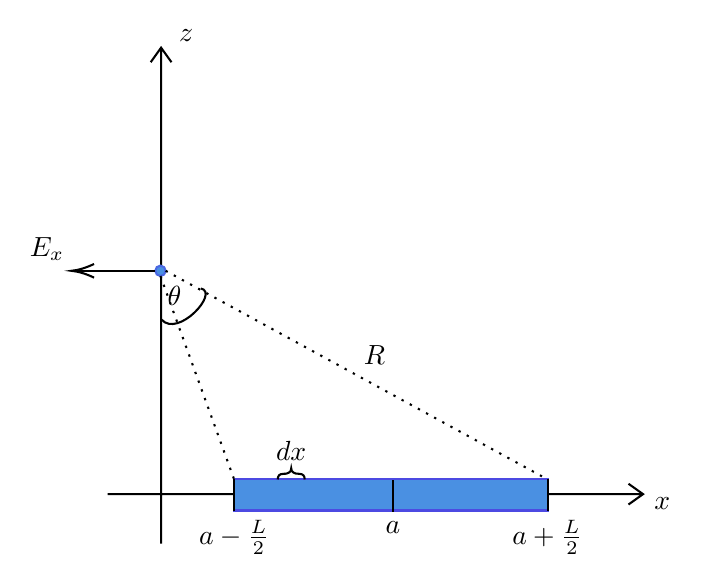
\begin{tikzpicture}[x=0.75pt,y=0.75pt,yscale=-1,xscale=1]
%uncomment if require: \path (0,430); %set diagram left start at 0, and has height of 430

%Shape: Axis 2D [id:dp24379060919610995] 
\draw  (189,279.1) -- (447,279.1)(214.8,64) -- (214.8,303) (440,274.1) -- (447,279.1) -- (440,284.1) (209.8,71) -- (214.8,64) -- (219.8,71)  ;
%Shape: Circle [id:dp5068074961038191] 
\draw  [color={rgb, 255:red, 74; green, 104; blue, 226 }  ,draw opacity=1 ][fill={rgb, 255:red, 74; green, 144; blue, 226 }  ,fill opacity=1 ] (212,171.5) .. controls (212,170.12) and (213.12,169) .. (214.5,169) .. controls (215.88,169) and (217,170.12) .. (217,171.5) .. controls (217,172.88) and (215.88,174) .. (214.5,174) .. controls (213.12,174) and (212,172.88) .. (212,171.5) -- cycle ;
%Shape: Rectangle [id:dp4049832220826315] 
\draw  [color={rgb, 255:red, 76; green, 74; blue, 226 }  ,draw opacity=1 ][fill={rgb, 255:red, 74; green, 144; blue, 226 }  ,fill opacity=1 ] (250,272) -- (401,272) -- (401,287) -- (250,287) -- cycle ;
%Straight Lines [id:da700289752662222] 
\draw  [dash pattern={on 0.84pt off 2.51pt}]  (217,171.5) -- (401,272) ;
%Straight Lines [id:da7713004879943914] 
\draw  [dash pattern={on 0.84pt off 2.51pt}]  (214.5,174) -- (250,272) ;
%Curve Lines [id:da724423688563848] 
\draw    (234,180) .. controls (243,182) and (223,204) .. (215,195) ;
%Straight Lines [id:da6170187006178778] 
\draw    (250,272) -- (250,287) ;
%Straight Lines [id:da0940078032787679] 
\draw    (401,272) -- (401,287) ;
%Straight Lines [id:da21330223589749187] 
\draw    (326.5,272.5) -- (326.5,287.5) ;
%Shape: Brace [id:dp2693887070076282] 
\draw   (284,272) .. controls (284,270.21) and (283.11,269.32) .. (281.32,269.32) -- (281.32,269.32) .. controls (278.77,269.32) and (277.5,268.43) .. (277.5,266.65) .. controls (277.5,268.43) and (276.23,269.32) .. (273.68,269.32)(274.82,269.32) -- (273.68,269.32) .. controls (271.89,269.32) and (271,270.21) .. (271,272) ;
%Straight Lines [id:da6088554153847827] 
\draw    (212,171.5) -- (173.58,171.5) ;
\draw [shift={(171.58,171.5)}, rotate = 360] [color={rgb, 255:red, 0; green, 0; blue, 0 }  ][line width=0.75]    (10.93,-3.29) .. controls (6.95,-1.4) and (3.31,-0.3) .. (0,0) .. controls (3.31,0.3) and (6.95,1.4) .. (10.93,3.29)   ;

% Text Node
\draw (222,62.6) node [anchor=south west] [inner sep=0.75pt]    {$z$};
% Text Node
\draw (451,279.4) node [anchor=north west][inner sep=0.75pt]    {$x$};
% Text Node
\draw (216.5,177.4) node [anchor=north west][inner sep=0.75pt]    {$\theta $};
% Text Node
\draw (311,218.35) node [anchor=south west] [inner sep=0.75pt]    {$R$};
% Text Node
\draw (250,290.4) node [anchor=north] [inner sep=0.75pt]    {$a-\frac{L}{2}$};
% Text Node
\draw (401,290.4) node [anchor=north] [inner sep=0.75pt]    {$a+\frac{L}{2}$};
% Text Node
\draw (326.5,290.9) node [anchor=north] [inner sep=0.75pt]    {$a$};
% Text Node
\draw (277.48,264.6) node [anchor=south] [inner sep=0.75pt]    {$dx$};
% Text Node
\draw (169.58,168.1) node [anchor=south east] [inner sep=0.75pt]    {$E_{x}$};


\end{tikzpicture}
